\documentclass[../mathNotesPreamble]{subfiles}
\begin{document}
%\relscale{1.4}
\tikzset{custNode/.style={color=black,inner sep=0.5pt,fill=none,opacity=1.0, text opacity=1}}
\tikzset{dLine/.style={mark=none, dashed, opacity=1.0, blue!85, line width=0.5pt}}
  \section{1.4: Trigonometric Functions and Their Inverses}
    \noindent
    \begin{minipage}[t]{0.6\linewidth}
      \begin{defn*}
        The \textbf{unit circle} is the circle of radius 1 that is centered at the origin.
      
        The angle corresponding to an arc length of 1 on a unit circle is called a \textbf{radian}.
      \end{defn*}
      A circle is $2\pi$ radians or $360^\circ$. Thus:
        \[2\pi=360^\circ \Longrightarrow 1=\dfrac{180^\circ}{\pi}=\dfrac{\pi}{180^\circ}\]
    \end{minipage}%
    \begin{minipage}[t]{0.4\linewidth}\ 
     
      \begin{flushright}
        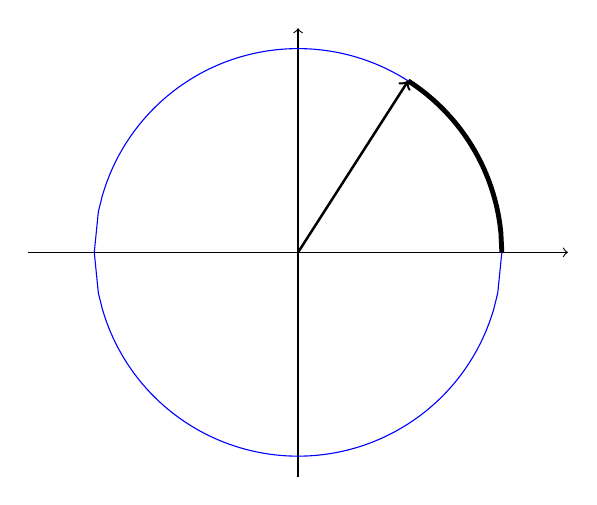
\begin{tikzpicture}[scale=1.0]
          \begin{axis}[
            axis lines=center,
            axis equal, 
            axis line style={->},
            xmin=-1.1, xmax=1.1,
            ymin=-1.1, ymax=1.1,
            xmajorticks=false,
            ymajorticks=false,
            ]
              \addplot[domain=-1:1, blue, samples=101] {sqrt(1-x^2)};
              \addplot[domain=0.5403:1, black, samples=101, line width=1.75pt] {sqrt(1-x^2)};
              \draw[->, black, line width = 0.9pt] (axis cs:0,0)--(axis cs:0.5403,0.84147);
              \addplot[domain=-1:1, blue, samples=101] {-sqrt(1-x^2)};
          \end{axis}
        \end{tikzpicture}
      \end{flushright}
    \end{minipage}

    \vfill
    \begin{defn*}
       The coordinates of a unit circle are given by $\parens{\cos(\theta),\sin(\theta)}$ for each $\theta$.
%    \end{defn*}
%    \begin{defn*}

      The $\sin(\theta)$ and $\cos(\theta)$ functions are \textbf{periodic} since these functions repeat themselves over a fixed interval.
    \end{defn*}
    \begin{center}
      \begin{tikzpicture}[scale=1.0]
        \begin{groupplot}[
          group style={group size=1 by 2}, 
          axis lines=center,
          axis line style={->},
          xmin=-7, xmax=7,
          ymin=-1.25, ymax=1.25,
          xtick={-6.28318, -4.7123889, ..., 6.28318},
          xticklabels={$-2\pi$, $-\frac{3\pi}{2}$,$-\pi$, $-\frac{\pi}{2}$, ,
             $\frac{\pi}{2}$,$\pi$, $\frac{3\pi}{2}$, $2\pi$},
          height=1.5in, width=0.95\linewidth,
          ticklabel style={font=\small, inner sep=0.75pt,fill=white},
          ]
          \nextgroupplot[xlabel=$\cos(\theta)$, xlabel style={at={(ticklabel* cs:1)},anchor=north west}]
            \addplot[domain=-6.28:6.28, blue, samples=101] {cos(deg(x))};
          \nextgroupplot[xlabel=$\sin(\theta)$, xlabel style={at={(ticklabel* cs:1)},anchor=north west}]
            \addplot[domain=-6.28:6.28, blue, samples=101] {sin(deg(x))};
        \end{groupplot}
      \end{tikzpicture}
    \end{center}
    \pagebreak
    
    \begin{defn*}
    
      Alternatively, $\cos(\theta)$ and $\sin(\theta)$ can be consider the ratio of the sides of a right angle triangle.
      
      \begin{minipage}{0.5\linewidth}
        \begin{tikzpicture}
          \draw (0,0) -- (8,0) -- (8,5) -- cycle;
          \draw (7.65,0) -- (7.65,0.35) -- (8,0.35);
          \node at (1,0.275) {$\theta$};
          \node at (4, -0.5) {Adj};
          \node at (8.55, 2.75) {Opp};
          \node at (4,3) {Hyp};
        \end{tikzpicture}
      \end{minipage}%
      \begin{minipage}{0.5\linewidth}
        \begin{align*}
          \sin\theta&=\dfrac{\textnormal{Opp}}{\textnormal{Hyp}}\\[10pt]
          \cos\theta&=\dfrac{\textnormal{Adj}}{\textnormal{Hyp}}\\[10pt]
          \tan\theta&=\dfrac{\textnormal{Opp}}{\textnormal{Adj}}\\[10pt]
        \end{align*}
      \end{minipage}
    \end{defn*}
    \begin{ex*}
      Find $\cos(\theta)$ and $\tan(\theta)$ given that $\sin(\theta)=\frac{3}{5}$ and $\pi/2\leq \theta\leq \pi$ (2nd quadrant).
    \end{ex*}
    
    \begin{minipage}{0.5\linewidth}
      \begin{tikzpicture}
        \draw (0,0) -- (8,0) -- (4,6.928) -- cycle;
        \draw[dashed] (4,0) -- (4,6.928);
        \draw (3.65,0) -- (3.65,0.35) -- (4,0.35);
        \node at (1.5,3.75) {1};
        \node at (6.5,3.75) {1};
        \node at (4,-0.5) {1};
      \end{tikzpicture}
    \end{minipage}%
    \begin{minipage}{0.5\linewidth}
      \begin{center}
        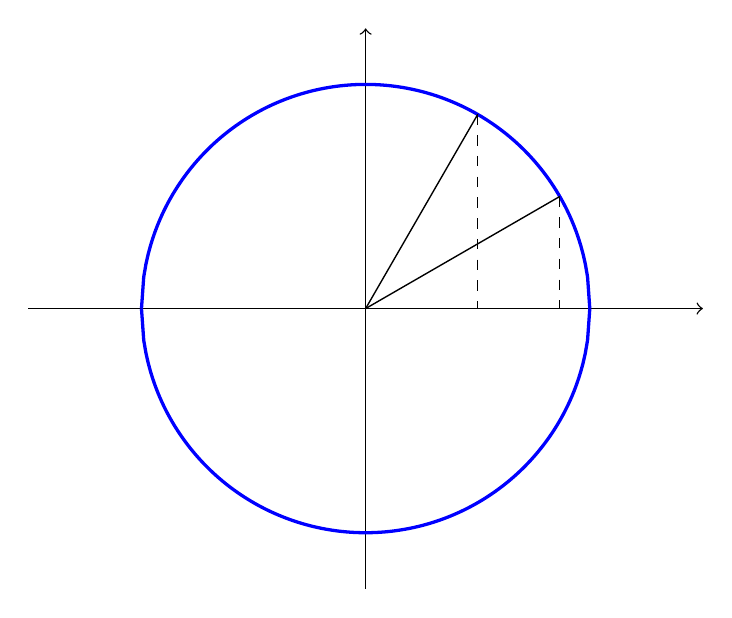
\begin{tikzpicture}[scale=1.25]
          \begin{axis}[
            axis lines=center,
            axis equal, 
            axis line style={->},
            ymin=-1.25, ymax=1.25,
            xmajorticks=false,
            ymajorticks=false,
            every axis plot/.append style={line width=0.95pt},
            ]
              \addplot[domain=-1:1, blue, samples=201] {sqrt(1-x^2)};
              \addplot[domain=-1:1, blue, samples=201] {-sqrt(1-x^2)};
              \draw (axis cs: 0,0) -- (axis cs: 0.5,0.866);
              \draw (axis cs: 0,0) -- (axis cs: 0.866,0.5);
              \draw[dashed] (axis cs: 0.866,0.5) -- (axis cs: 0.866,0);
              \draw[dashed] (axis cs: 0.5,0.866) -- (axis cs: 0.5,0);
          \end{axis}
        \end{tikzpicture}
      \end{center}
    \end{minipage}
    
    \vspace*{\stretch{1}}
    \begin{minipage}{0.475\linewidth}
      \begin{tikzpicture}[scale=0.85]
        \draw (0,0) -- (8,0) -- (8,8) -- cycle;
        \draw (7.65,0) -- (7.65,0.35) -- (8,0.35);
        \node at (4,4.5) {1};
        \node at (8.5,4) {$s$};
        \node at (4,-0.5) {$s$};
      \end{tikzpicture}
    \end{minipage}%
    \begin{minipage}{0.5\linewidth}
      \begin{center}
        \begin{tikzpicture}[scale=1.25]
          \begin{axis}[
            axis lines=center,
            axis equal, 
            axis line style={->},
            ymin=-1.25, ymax=1.25,
            xmajorticks=false,
            ymajorticks=false,
            every axis plot/.append style={line width=0.95pt},
            ]
              \addplot[domain=-1:1, blue, samples=201] {sqrt(1-x^2)};
              \addplot[domain=-1:1, blue, samples=201] {-sqrt(1-x^2)};
              \draw (axis cs: 0,0) -- (axis cs: 0.707,0.707);
              \draw[dashed] (axis cs: 0.707,0.707) -- (axis cs: 0.707,0);
          \end{axis}
        \end{tikzpicture}
      \end{center}
    \end{minipage}
    \pagebreak
    
    \vspace*{\stretch{0.75}}
    \begin{center}
      \newcommand{\rRad}{0.875}
      \newcommand{\cRad}{1.2}
      \newcommand{\lCol}{gray!90}
      \begin{tikzpicture}[scale=7.0]
        \draw[line width=1pt] (0,0) circle(1);
        \foreach \x in {0,30,...,360} {
        \draw[\lCol] (0cm,0cm) -- (\x:1);
        }
        
        \foreach \x in {45,135,225,315} {
          \draw[\lCol] (0cm,0cm) -- (\x:1);
          }
        \ifprintanswers\foreach \x/\xtext in {
          30/\dfrac{\pi}{6},
          45/\dfrac{\pi}{4},
          60/\dfrac{\pi}{3}}
          \draw (\x:\rRad) node[fill=white] {$\xtext$};
      \foreach \x/\xtext/\y in {
        30/\frac{\sqrt{3}}{2}/\frac{1}{2},
        45/\frac{\sqrt{2}}{2}/\frac{\sqrt{2}}{2},
        60/\frac{1}{2}/\frac{\sqrt{3}}{2}}
          \draw (\x:\cRad) node {$\left(\xtext,\y\right)$};
      \draw (-\cRad,0cm) node{$(-1,0)$}
            (\cRad,0cm)  node{$(1,0)$}
            (0cm,-\cRad) node{$(0,-1)$}
            (0cm,\cRad)  node{$(0,1)$};\fi
      \end{tikzpicture}
    \end{center}
    
    \vspace*{\stretch{1}}
    \pagebreak

    \noindent
    There are 6 trig functions, all of which can be written in terms of $\sin(\theta)$ and $\cos(\theta)$:
    
    \[\begin{array}{r@{\ =\ }l@{\hspace*{2in}}r@{\ =\ }l}
      \tan\theta&\hphantom{\dfrac{\sin\theta}{\cos\theta}}&
      \cot\theta&\hphantom{\dfrac{\cos\theta}{\sin\theta}}\\[20pt]
      \sec\theta&&
      \csc\theta&
    \end{array}\]
    \vspace*{\stretch{1}}
    
    \noindent
    These functions can also be represented with the sides of a right triangle:
    \vspace*{10pt}    
    
    \begin{minipage}{0.45\linewidth}
      \begin{tikzpicture}[scale=0.85]
        \draw (0,0) -- (8,0) -- (8,5) -- cycle;
        \draw (7.65,0) -- (7.65,0.35) -- (8,0.35);
        \node at (1,0.275) {$\theta$};
        \node at (4, -0.5) {Adj};
        \node at (8.75, 2.75) {Opp};
        \node at (4,3.125) {Hyp};
      \end{tikzpicture}
    \end{minipage}%
    \begin{minipage}{0.5\linewidth}
      $\begin{array}{@{}r@{\ =\ }@{\hspace*{1.0in}}r@{\ =\ }}
        \tan\theta& \cot\theta\\[40pt]
        \sec\theta& \csc\theta
      \end{array}$
      \vspace*{25pt}
    \end{minipage}

    \vspace*{\stretch{1}}
    \noindent
    Using these functions, we have the following Pythagorean Identities:
    \begin{center}
      \renewcommand{\arraystretch}{1.5}
      \begin{tabular}{C@{ + }C@{ = }L}
        \sin^2(\theta)&\cos^2(\theta)&1\\
        \tan^2(\theta)&1&\underline{\hspace*{1.5in}}\\
        1&\cot^2(\theta)&\underline{\hspace*{1.5in}}
      \end{tabular}
    \end{center}
    
    \begin{ex*}
      Show the identity: $\tan\theta+\cot\theta=\sec\theta\csc\theta$.
    \end{ex*}
    \vspace*{\stretch{1}}
    \pagebreak

    \begin{defn*}
      The \textbf{Angle Sum Formulas} are
      \begin{align*}
        \sin(A\pm B)&=\sin(A)\cos(B)\pm\cos(A)\sin(B)\\
        \cos(A\pm B)&=\cos(A)\cos(B)\mp\sin(A)\sin(B)
      \end{align*}
      \textbf{Note:} Since $\cos(\theta)$ is even and $\sin(\theta)$ is odd, we can derive the difference formula from the sum formula.
    \end{defn*}
    \vspace*{15pt}

    \begin{defn*}
      The \textbf{double-angle formulas} are a special case of the angle-sum formulas:
      \begin{minipage}{0.5\linewidth}
        \begin{align*}
          \sin(2\theta)&=\sin(\theta+\theta)\\
            &=\sin(\theta)\cos(\theta)+\cos(\theta)\sin(\theta)\\
            &=\boxed{2\sin(\theta)\cos(\theta)}
        \end{align*}
      \end{minipage}%
      \begin{minipage}{0.5\linewidth}
        \begin{align*}
          \cos(2\theta)&=\cos(\theta+\theta)\\
            &=\cos(\theta)\cos(\theta)-\sin(\theta)\sin(\theta)\\
            &=\boxed{\cos^2(\theta)-\sin^2(\theta)}
        \end{align*}
      \end{minipage}\\[15pt]

    \textbf{Note:} Using the Pythagorean Identity, we have 2 additional representations of $\cos(2\theta)$.
    \end{defn*}

    \begin{ex*}
      Evaluate $\sin\parens{\frac{2\pi}{3}}$ using the double-angle formula.
    \end{ex*}
    \vspace*{\stretch{1}}
    \pagebreak

    \begin{defn*}
      The \textbf{half-angle formulas} are derived from the double angle formula:
      \begin{align*}
        \sin(\theta)&=\pm\sqrt{\frac{1-\cos(2\theta)}{2}}\\
        \cos(\theta)&=\pm\sqrt{\frac{1+\cos(2\theta)}{2}}
      \end{align*}
    \end{defn*}
    \begin{ex*}
      Evaluate $\cos\parens{\frac{\pi}{12}}$ using the half-angle formula.
    \end{ex*}
    \vspace*{\stretch{1}}
    
    \begin{ex*}
      Solve the following equation:
    \end{ex*}
      \[\cos(3\theta)=\sin(3\theta),\quad 0\leq\theta< 2\pi\]
    \vspace*{\stretch{1}}
    \pagebreak

    \vspace*{\stretch{1}}
    \begin{center}
      \begin{tikzpicture}
        \begin{groupplot}[
          group style={group size=2 by 2, horizontal sep=1.25cm, vertical sep=2cm},
          axis lines=center,
          axis line style={->},
          xmin=-1.5, xmax=4*pi+1.25,
          ymin=-3, ymax=3,
          xtick={1.570796327,3.141592654,...,12.566370614},
          xticklabels={$\frac{\pi}{2}$,$\pi$,$\frac{3\pi}{2}$,$2\pi$,$\frac{5\pi}{2}$,$3\pi$,$\frac{7\pi}{2}$,$4\pi$},
          ytick={-2,-1,...,2},
          yticklabels={,-1,,1,},
          ticklabel style={font=\footnotesize,inner sep=0.5pt,fill=white,opacity=1.0, text opacity=1},
          width=0.5\linewidth,
          every axis plot/.append style={line width=0.95pt, color=blue, samples=501}
          ]
            \nextgroupplot
              \addplot[-] expression[domain=-1.5:4*pi+1.25, ClemsonPurple] {sin(\x*180/pi)};
              \addlegendentry{$\sin(\theta)$};
              \foreach \k in {0,1,...,5}{
                \addplot[-] expression[domain=(\k-1)*pi+0.1:\k*pi-0.1, unbounded coords=discard, ClemsonOrange] {1/sin(\x*180/pi)};
                \addplot +[dashed, black!50, line width=0.5pt, mark=none] coordinates{((\k+1)*pi,-3)((\k+1)*pi,3)};
              }
              \addlegendentry{$\csc(\theta)$};
            \nextgroupplot
              \addplot[-] expression[domain=-1.5:4*pi+1.25, ClemsonPurple] {cos(\x*180/pi)};
              \addlegendentry{$\cos(\theta)$};
              \foreach \k in {0,1,...,5}{
                \addplot[-] expression[domain=(2*\k-1)*pi/2+0.1:(2*\k+1)*pi/2-0.1, unbounded coords=discard, ClemsonOrange] {1/cos(\x*180/pi)};
                \addplot +[dashed, black!50, line width=0.5pt, mark=none] coordinates{((2*\k+1)*pi/2,-3)((2*\k+1)*pi/2,3)};
              }
              \addlegendentry{$\sec(\theta)$};
            \nextgroupplot
              \foreach \k in {0,1,...,5}{
                \addplot[-] expression[domain=(2*\k-1)*pi/2+0.1:(2*\k+1)*pi/2-0.1, unbounded coords=discard, ClemsonPurple] {tan(\x*180/pi)};
                \addplot +[dashed, black!50, line width=0.5pt, mark=none] coordinates{((2*\k+1)*pi/2,-3)((2*\k+1)*pi/2,3)};
}
              \addlegendentry{$\tan(\theta)$};
            \nextgroupplot
              \foreach \k in {0,1,...,5}{
                \addplot[-] expression[domain=(\k-1)*pi+0.1:\k*pi-0.1, unbounded coords=discard, ClemsonPurple] {cot(\x*180/pi)};
                \addplot +[dashed, black!50, line width=0.5pt, mark=none] coordinates{((\k+1)*pi,-3)((\k+1)*pi,3)};
}
              \addlegendentry{$\cot(\theta)$};
        \end{groupplot}
      \end{tikzpicture}
    \end{center}
    \vspace*{\stretch{1}}
    \pagebreak

    Recall that a function has an inverse if it is 1-to-1 (e.g. it passes the horizontal line test).
  \begin{center}
    \begin{tikzpicture}
      \begin{groupplot}[
        group style={group size=3 by 1, horizontal sep=1cm},
        width=0.36\linewidth,
        axis lines=center,
        axis line style={->},
        ticklabel style={font=\footnotesize,inner sep=0.5pt,fill=white,opacity=1.0, text opacity=1},
        xlabel=$x$, xlabel style={at={(ticklabel* cs:1)},anchor=north west},
        ylabel=$y$, ylabel style={at={(ticklabel* cs:1)},anchor=south west},
        every axis plot/.append style={line width=0.95pt, color=blue}
        ]
        \nextgroupplot[
          xmin=-4.25, xmax=6.25,
          ymin=-4.25, ymax=6.25,
          xmajorticks=false,
          ymajorticks=false,
          every axis plot/.append style={samples=100},
          ]
          \addplot[dashed] expression[domain=-4.25:6.25, black]{x};
          \addplot[->] expression[domain=-4.25:ln(6.25), ClemsonPurple] {e^x} node[custNode, below right, pos=1] {$a^x$};
          \addplot[->] expression[domain=exp(-4.25):6.25, ClemsonOrange] {ln(x)} node[custNode, above left, pos=1] {$\log_a(x)$};
        \nextgroupplot[
          xmin=-0.5, xmax=3.25,
          ymin=-0.5, ymax=3.25,
          xmajorticks=false,
          ymajorticks=false,
          every axis plot/.append style={samples=500},
          ]
          \addplot[dashed] expression[domain=-0.5:3.25, black]{x};
          \addplot[dashed] expression[domain=-0.5:0, ClemsonPurple]{x^2};
          \addplot[->] expression[domain=0:sqrt(3.25), ClemsonPurple]{x^2} node[custNode, below right, pos=1] {$x^2$};
          \addplot[->] expression[domain=0:3.25, ClemsonOrange]{sqrt(x)} node[custNode, above left, pos=1] {$\sqrt x$};
        \nextgroupplot[
          xmin=-(pi/2+0.5), xmax=(pi/2+0.775),
          ymin=-(pi/2+0.5), ymax=(pi/2+0.65),
          xmajorticks=false,
          ymajorticks=false,
          every axis plot/.append style={samples=100},
          ]
          \addplot[dashed] expression[domain=-(pi/2+0.5):(pi/2+0.775), black]{x};
          \addplot[dashed] expression[domain=-pi/2-0.5:-pi/2, ClemsonPurple]{sin(x*180/pi)};
          \addplot[dashed] expression[domain=pi/2:pi/2+0.775, ClemsonPurple]{sin(x*180/pi)};
          \addplot[-] expression[domain=-pi/2:pi/2, ClemsonPurple]{sin(x*180/pi)} node[custNode, below right, pos=0.85] {$\sin(x)$};
          \addplot[-] expression[domain=-1:1, ClemsonOrange]{asin(x)*pi/180} node[custNode, above, pos=1, xshift=-5pt] {$\arcsin(x)$};
      \end{groupplot}
    \end{tikzpicture}
    
    Notice that $x^2$ and $\sin(x)$ are on restricted domains.
  \end{center}

Without restriction on its domain, $\sin(x)$ is NOT 1-to-1:
\begin{center}
  \begin{tikzpicture}
    \begin{axis}[
      axis lines=center,
      axis line style={->},
      xmin=-7, xmax=7,
      ymin=-1.25, ymax=1.25,
      xtick={-6.28318, -4.7123889, ..., 6.28318},
      xticklabels={$-2\pi$, $-\frac{3\pi}{2}$,$-\pi$, $-\frac{\pi}{2}$, ,
         $\frac{\pi}{2}$,$\pi$, $\frac{3\pi}{2}$, $2\pi$},
      height=1.75in, width=0.9\linewidth,
      ticklabel style={font=\small, inner sep=0.75pt,fill=white},
      xlabel=$x$, xlabel style={at={(ticklabel* cs:1)},anchor=north west},
      ylabel=$y$, ylabel style={at={(ticklabel* cs:1)},anchor=south west},
      every axis plot/.append style={line width=0.95pt, color=blue}
      ]
      \addplot[domain=-6.28:6.28, ClemsonPurple, samples=101] {sin(deg(x))} node[custNode, pos=0.7, above right] {$\sin(x)$};
    \end{axis}
  \end{tikzpicture}
\end{center}

The range of $\sin(x)$ is $[-1,1]$ and all of these values are attained on a restricted domain of $\sbrkt{\nicefrac{-\pi}{2},\nicefrac{\pi}{2}}$:

\begin{center}
  \begin{tikzpicture}
    \begin{groupplot}[
      group style={group size=2 by 1, horizontal sep=4cm},
      axis lines=center,
      axis line style={->},
      xmin=-(pi/2+0.95), xmax=pi/2+0.95,
      ymin=-(pi/2+0.95), ymax=pi/2+0.95,
      width=0.4\linewidth,
      ticklabel style={font=\small, inner sep=0.75pt,fill=white},
      xlabel=$x$, xlabel style={at={(ticklabel* cs:1)},anchor=north west},
      ylabel=$y$, ylabel style={at={(ticklabel* cs:1)},anchor=south west},
      every axis plot/.append style={line width=0.95pt, color=blue, samples=100}      
      ]
      \nextgroupplot[
        xtick={-1.570796327,1.570796327},
        ytick={-1,1},
        xticklabels={$-\frac{\pi}{2}$,$\frac{\pi}{2}$},
        ]
        \addplot[-] expression[domain=-pi/2:pi/2, ClemsonPurple]{sin(x*180/pi)};
        \node[custNode] at (-pi/2,1) {$\sin(x)$};
        \addplot[soldot, black] coordinates{(-pi/2,-1)} node[custNode, below, xshift=5pt, yshift=-4pt] {$\parens{\frac{-\pi}{2},-1}$};
        \addplot[soldot, black] coordinates{(pi/2,1)} node[custNode, above, xshift=5pt, yshift=4pt] {$\parens{\frac{\pi}{2},1}$};
      \nextgroupplot[
        xtick={-1,1},
        ytick={-1.570796327,1.570796327},
        yticklabels={$-\frac{\pi}{2}$,$\frac{\pi}{2}$},
        ]
        \addplot[-] expression[domain=-1:1, ClemsonOrange]{asin(x)*pi/180};
        \node[custNode] at (-pi/2,1) {$\arcsin(x)$};
        \addplot[soldot, black] coordinates{(-1,-pi/2)} node[custNode, below left] {$\parens{-1,\frac{-\pi}{2}}$};
        \addplot[soldot, black] coordinates{(1,pi/2)} node[custNode, above right] {$\parens{1,\frac{\pi}{2}}$};
    \end{groupplot}
  \end{tikzpicture}
\end{center}
  \pagebreak
  
  \begin{defn*}[Inverse Sine and Cosine]
    \def\tmp{5pt}
    $y=\sin\inv(x)$ is the value of $y$ such that $x=\sin(y)$, where $\nicefrac{-\pi}{2}\leq y\leq \nicefrac{\pi}{2}$.\\[\tmp]
    $y=\cos\inv(x)$ is the value of $y$ such that $x=\cos(y)$, where $0\leq y\leq \pi$.\\[\tmp]
    The domain of both $\sin\inv(x)$ and $\cos\inv(x)$ is $\set{x\mid -1\leq x\leq 1}$.
  \end{defn*}

  \textit{Note}: The inverse sine function can be denoted as $\arcsin(x)$ or $\sin\inv(x)$.
  
  This means that $\sin\inv(x)\neq \dfrac{1}{\sin(x)}$. 
  
  Similarly, $\arccos(x)$ and $\cos\inv(x)$ denote the inverse cosine functions.
  \vfill
\begin{center}
  \begin{tikzpicture}
    \begin{groupplot}[
      group style={group size=2 by 1, horizontal sep=2cm},
      axis lines=center,
      axis line style={->},
      width=0.45\linewidth,
      ticklabel style={font=\small, inner sep=0.75pt,fill=white},
      xlabel=$x$, xlabel style={at={(ticklabel* cs:1)},anchor=north west},
      ylabel=$y$, ylabel style={at={(ticklabel* cs:1)},anchor=south west},
      every axis plot/.append style={line width=0.95pt, color=blue, samples=100}      
      ]
      \nextgroupplot[
        xmin=-(pi/2+0.95), xmax=pi/2+0.95,
        ymin=-(pi/2+0.95), ymax=pi/2+0.95,
        xtick={-1.570796327,-1,1,1.570796327},
        ytick={-1.570796327,-1,1,1.570796327},
        xticklabels={$-\frac{\pi}{2}$,-1,1,$\frac{\pi}{2}$},
        yticklabels={$-\frac{\pi}{2}$,-1,1,$\frac{\pi}{2}$},
        ]
        \addplot[-] expression[domain=-pi/2:pi/2, ClemsonPurple]{sin(x*180/pi)} node[custNode, below right, pos=0.95] {$\sin(x)$};
        \addplot[-] expression[domain=-1:1, ClemsonOrange]{asin(x)*pi/180} node[custNode, above, pos=1] {$\sin\inv(x)$};
      \nextgroupplot[
        xmin=-1.5, xmax=pi+0.95,
        ymin=-1.5, ymax=pi+0.95,
        xtick={-1,1,3.141592654},
        ytick={-1,1,3.141592654},
        xticklabels={-1,1,$\pi$},
        yticklabels={-1,1,$\pi$},
        ]
        \addplot[-] expression[domain=0:pi, ClemsonPurple]{cos(x*180/pi)} node[custNode, above right, pos=0.95] {$\cos(x)$};
        \addplot[-] expression[domain=-1:1, ClemsonOrange]{acos(x)*pi/180} node[custNode, above, pos=0.0, xshift=7.5pt, yshift=2.5pt] {$\cos\inv(x)$};
    \end{groupplot}
  \end{tikzpicture}
\end{center}
  \vfill
  \begin{ex*}
    Solve the following:
  \end{ex*}
  \begin{tasks}[after-item-skip=\stretch{1}, label=~](3)
    \task $\sin\inv(0)$
    \task $\arcsin(1)$
    \task $\sin\inv\parens{\dfrac{\sqrt 3}{2}}$
    \task $\cos\inv\parens{-1}$
    \task $\cos\inv\parens{-\dfrac{1}{2}}$
    \task $\arccos\parens{-\dfrac{\sqrt3}{2}}$
  \end{tasks}
  \vfill 
  \pagebreak

  \begin{defn*}[Inverse Tangent and Secant]
    \def\tmp{5pt}
    $y=\tan\inv(x)$ is the value of $y$ such that $x=\tan(y)$, where $\nicefrac{-\pi}{2}< y< \nicefrac{\pi}{2}$.\\[\tmp]
    The domain of $\tan\inv(x)$ is $\set{x\mid -\infty< x< \infty}$.\\[\tmp]
    $y=\sec\inv(x)$ is the value of $y$ such that $x=\sec(y)$, where $0\leq y\leq \pi,\  y\neq\nicefrac{\pi}{2}$.\\[\tmp]
    The domain of $\sec\inv(x)$ is $(-\infty,-1]\cup[1,\infty)$
  \end{defn*}

\vfill
  
\begin{center}
  \def\arraystretch{1.5}\tabcolsep=15pt
  \begin{tabular}{@{}LCC@{}}\toprule
    \textnormal{Function}& \lnret[c]{Restricted\\[-10pt]Domain}& \textnormal{Range}\\\midrule
    \sin(x)& [\nicefrac{-\pi}{2},\nicefrac{\pi}{2}]& [-1,1]\\
    \cos(x)& [0,\pi]& [-1,1]\\
    \tan(x)& \parens{\nicefrac{-\pi}{2},\nicefrac{\pi}{2}}& (-\infty,\infty)\\
    \cot(x)& (0,\pi)& (-\infty,\infty)\\
    \sec(x)& [0,\nicefrac{\pi}{2})\cup (\nicefrac{\pi}{2},\pi]& (-\infty,-1]\cup[1,\infty)\\
    \csc(x)& [\nicefrac{-\pi}{2},0)\cup(0,\nicefrac{\pi}{2}]& (-\infty,-1]\cup[1,\infty)\\\bottomrule
  \end{tabular}
\end{center}  
\vfill

\begin{center}
  \def\arraystretch{1.5}\tabcolsep=15pt
  \begin{tabular}{@{}LCC@{}}\toprule
   \textnormal{Function}& \textnormal{Domain}& \textnormal{Range}\\\midrule
    \sin\inv(x) &  [-1,1] &  [\nicefrac{-\pi}{2},\nicefrac{\pi}{2}] \\
    \cos\inv(x) &  [-1,1] &  [0,\pi] \\
    \tan\inv(x) &  (-\infty,\infty) &  \parens{\nicefrac{-\pi}{2},\nicefrac{\pi}{2}} \\
    \cot\inv(x) &  (-\infty,\infty) &  (0,\pi) \\
    \sec\inv(x) &  (-\infty,-1]\cup[1,\infty) &  [0,\nicefrac{\pi}{2})\cup (\nicefrac{\pi}{2},\pi]\\
    \csc\inv(x) &  (-\infty,-1]\cup[1,\infty) &  [\nicefrac{-\pi}{2},0)\cup(0,\nicefrac{\pi}{2}] \\
\bottomrule
  \end{tabular}
\end{center}
\vfill
\pagebreak
\vfill

\begin{center}
  \begin{tikzpicture}[declare function={
    limOne=4; limTwo=4; limThree=4; limFour=4;}]
    \begin{groupplot}[
      group style={group size=2 by 3, horizontal sep=2cm},
      width=0.44\linewidth,
      axis lines=center,
      axis line style={->},
      ticklabel style={font=\footnotesize,inner sep=0.5pt,fill=white,opacity=1.0, text opacity=1},
      xlabel=$x$, xlabel style={at={(ticklabel* cs:1)},anchor=north west},
      ylabel=$y$, ylabel style={at={(ticklabel* cs:1)},anchor=south west},
      every axis plot/.append style={line width=0.95pt, color=blue, samples=100}
      ]
%%%%%%%%%%%%%%%%%%%%%%%%%%%%%%%%%%%%%%%%%%%%%%%%%%%%%%%%%%%%%%%%%%%%%%%%%%%%%%%
      \nextgroupplot[
        xmin=-(pi/2+0.95), xmax=pi/2+0.95,
        ymin=-(pi/2+0.95), ymax=pi/2+0.95,
        xtick={-pi/2,-1,1,pi/2},
        ytick={-pi/2,-1,1,pi/2},
        xticklabels={$-\frac{\pi}{2}$,-1,1,$\frac{\pi}{2}$},
        yticklabels={$-\frac{\pi}{2}$,-1,1,$\frac{\pi}{2}$},
        ]
        \addplot[dLine] coordinates {(-1,-limOne) (-1,limOne)};
        \addplot[dLine] coordinates {(1,-limOne) (1,limOne)};
        \addplot[dLine] coordinates {(-limOne,1) (limOne,1)};
        \addplot[dLine] coordinates {(-limOne,-1) (limOne,-1)};
        \addplot[-] expression[domain=-pi/2:pi/2,
          ClemsonPurple]{sin((x) r)} node[custNode, below right,
          pos=0.95] {$\sin(x)$};
        \addplot[-] expression[domain=-1:1,
          ClemsonOrange]{asin(x)*pi/180} node[custNode, above, pos=1]
          {$\sin\inv(x)$};
%%%%%%%%%%%%%%%%%%%%%%%%%%%%%%%%%%%%%%%%%%%%%%%%%%%%%%%%%%%%%%%%%%%%%%%%%%%%%%%
      \nextgroupplot[
        xmin=-1.5, xmax=pi+0.95,
        ymin=-1.5, ymax=pi+0.95,
        xtick={-1,1,pi},
        ytick={-1,1,pi},
        xticklabels={-1,1,$\pi$},
        yticklabels={-1,1,$\pi$},
        ]
        \addplot[dLine] coordinates {(-1,-limTwo) (-1,limTwo)};
        \addplot[dLine] coordinates {(1,-limTwo) (1,limTwo)};
        \addplot[dLine] coordinates {(-limTwo,1) (limTwo,1)};
        \addplot[dLine] coordinates {(-limTwo,-1) (limTwo,-1)};
        \addplot[-] expression[domain=0:pi,
          ClemsonPurple]{cos((x) r)} node[custNode, above right,
          pos=0.95] {$\cos(x)$};
        \addplot[-] expression[domain=-1:1,
          ClemsonOrange]{acos(x)*pi/180} node[custNode, above,
          pos=0.0, xshift=7.5pt, yshift=2.5pt] {$\cos\inv(x)$};
%%%%%%%%%%%%%%%%%%%%%%%%%%%%%%%%%%%%%%%%%%%%%%%%%%%%%%%%%%%%%%%%%%%%%%%%%%%%%%%
      \nextgroupplot[
        xmin=-limOne, xmax=limOne,
        ymin=-limOne, ymax=limOne,
        xtick={-pi/2,-1,1,pi/2},
        ytick={-pi/2,-1,1,pi/2},
        xticklabels={$-\frac{\pi}{2}$,-1,1,$\frac{\pi}{2}$},
        yticklabels={$-\frac{\pi}{2}$,-1,1,$\frac{\pi}{2}$},
        ]
        \addplot[dLine] coordinates {(-pi/2,-limTwo) (-pi/2,limTwo)};
        \addplot[dLine] coordinates {(pi/2,-limTwo) (pi/2,limTwo)};
        \addplot[dLine] coordinates {(-limTwo,pi/2) (limTwo,pi/2)};
        \addplot[dLine] coordinates {(-limTwo,-pi/2) (limTwo,-pi/2)};
        \addplot[-] expression[domain=-1.32:1.32,
          ClemsonPurple]{tan((x) r)} node[custNode, right, pos=0.95,
          xshift=7pt] {$\tan(x)$};
        \addplot[-] expression[domain=-limOne:limOne,
          ClemsonOrange]{atan(x)*pi/180} node[custNode, below right,
          pos=0.75] {$\tan\inv(x)$};
%%%%%%%%%%%%%%%%%%%%%%%%%%%%%%%%%%%%%%%%%%%%%%%%%%%%%%%%%%%%%%%%%%%%%%%%%%%%%%%
      \nextgroupplot[
        xmin=-limThree, xmax=limThree,
        ymin=-limThree, ymax=limThree,
        xtick={-1,1,pi},
        ytick={-1,1,pi},
        xticklabels={-1,1,$\pi$},
        yticklabels={-1,1,$\pi$},
        ]
        \addplot[dLine] coordinates {(0,-limTwo) (0,limTwo)};
        \addplot[dLine] coordinates {(pi,-limTwo) (pi,limTwo)};
        \addplot[dLine] coordinates {(-limTwo,0) (limTwo,0)};
        \addplot[dLine] coordinates {(-limTwo,pi) (limTwo,pi)};
        \addplot[-] expression[domain=0.25:3,
          ClemsonPurple]{cot((x) r)} node[custNode, right, pos=0.1,
          xshift=5pt] {$\cot(x)$};
        \addplot[-] expression[domain=-limThree:-0.0001, ClemsonOrange]{atan(1/x)*pi/180+pi};
        \addplot[-] expression[domain=0.0001:limThree,
          ClemsonOrange]{atan(1/x)*pi/180} node[custNode, above,
          pos=0.725] {$\cot\inv(x)$};
%%%%%%%%%%%%%%%%%%%%%%%%%%%%%%%%%%%%%%%%%%%%%%%%%%%%%%%%%%%%%%%%%%%%%%%%%%%%%%%        
      \nextgroupplot[
        xmin=-limTwo, xmax=limTwo,
        ymin=-limTwo, ymax=limTwo,
        xtick={-pi/2,-1,1,pi/2,pi},
        ytick={-pi/2,-1,1,pi/2,pi},
        xticklabels={$-\frac{\pi}{2}$,-1,1,$\frac{\pi}{2}$,$\pi$},
        yticklabels={$-\frac{\pi}{2}$,-1,1,$\frac{\pi}{2}$,$\pi$},
        ]
        \addplot[dLine] coordinates {(pi/2,-limTwo) (pi/2,limTwo)};
        \addplot[dLine] coordinates {(-limTwo,pi/2) (limTwo,pi/2)};
        \addplot[-] expression[domain=0:1.5,
        ClemsonPurple]{1/cos((x) r)} node[custNode, right,
          pos=0.225, xshift=7.5pt] {$\sec(x)$};
        \addplot[-] expression[domain=1.7:pi,
          ClemsonPurple]{1/cos((x) r)};
        \addplot[-] expression[domain=-limTwo:-1,
          ClemsonOrange]{acos(1/x)*pi/180};
        \addplot[-] expression[domain=1:limTwo,
          ClemsonOrange]{acos(1/x)*pi/180} node[custNode, below,
          pos=0.725] {$\sec\inv(x)$};
%%%%%%%%%%%%%%%%%%%%%%%%%%%%%%%%%%%%%%%%%%%%%%%%%%%%%%%%%%%%%%%%%%%%%%%%%%%%%%%
      \nextgroupplot[ 
        xmin=-limFour, xmax=limFour,
        ymin=-limFour, ymax=limFour,
        xtick={-pi/2,-1,1,pi/2,pi},
        ytick={-pi/2,-1,1,pi/2,pi},
        xticklabels={$-\frac{\pi}{2}$,-1,1,$\frac{\pi}{2}$,$\pi$},
        yticklabels={$-\frac{\pi}{2}$,-1,1,$\frac{\pi}{2}$,$\pi$},
        ]
        \addplot[dLine] coordinates {(0,-limTwo) (0,limTwo)};
        \addplot[dLine] coordinates {(-limTwo,0) (limTwo,0)};
        \addplot[-] expression[domain=-1.5:-0.25, ClemsonPurple]{1/sin((x) r)};
        \addplot[-] expression[domain=0.25:1.5,
          ClemsonPurple]{1/sin((x) r)} node[custNode, right,
          pos=0.225, xshift=7.5pt] {$\csc(x)$};
        \addplot[-] expression[domain=-limFour:-1,
          ClemsonOrange]{asin(1/x)*pi/180};
        \addplot[-] expression[domain=1:limFour,
          ClemsonOrange]{asin(1/x)*pi/180} node[custNode, above,
          pos=0.725] {$\csc\inv(x)$};
%%%%%%%%%%%%%%%%%%%%%%%%%%%%%%%%%%%%%%%%%%%%%%%%%%%%%%%%%%%%%%%%%%%%%%%%%%%%%%%
    \end{groupplot}
  \end{tikzpicture}
\end{center}

\vfill
  \pagebreak
  \begin{ex*}
    Solve the following:
  \end{ex*}
  \begin{tasks}[label=~](3)
    \task $\sin\inv\parens{-\frac{1}{\sqrt{2}}}$
    \task $\sec\inv(2)$
    \task $\cot\inv\parens{-\sqrt{3}}$
  \end{tasks}
  \vspace*{15pt}

  While $\sin(x)$ and $\sin\inv(x)$ are inverse functions, the inverse relationship only holds when working in the correct domains:
  \begin{tasks}[label=~](2)
    \task $\sin\inv\parens{\sin(\pi)}=\sin\inv(0)=0\neq \pi$
    \task $\sin\parens{\sin\inv(-1)}=\sin\parens{\nicefrac{-\pi}{2}}=-1$
  \end{tasks}
  \vspace*{15pt}
  \begin{ex*}
    Solve the following:
  \end{ex*}
    \begin{tasks}[after-item-skip=\stretch{1}, label=~](2)
      \task $\tan(\tan\inv(5))$
      \task $\tan\inv\parens{\tan\dfrac{3\pi}{4}}$
      \task $\cos\parens{\arcsin\dfrac{1}{2}}$
      \task $\cos\inv\parens{\cos(5\pi)}$
    \end{tasks}
  \vfill
  \pagebreak
  
  \begin{tasks}[after-item-skip=\stretch{1}, label=~](3)
    \task $\sin\inv\parens{\sin\parens{\dfrac{7\pi}{3}}}$
    \task $\tan\parens{\sec\inv(10)}$
    \task $\sin\parens{2\sin\inv\parens{\dfrac{3}{5}}}$
  \end{tasks}
    \vfill
  \begin{ex*}
    Simplify the following using triangles.
  \end{ex*}
  \begin{tasks}[after-item-skip=\stretch{1}, label=~](1)
    \task $\cos\parens{\tan\inv(x)}$
    \task $\sec\parens{\sin\inv(x)}$
    \task $\cos\parens{2\sin\inv(x)}$
    \task $\sin\parens{2\tan\inv(x)}$
  \end{tasks}
  \vfill
  \pagebreak
\end{document}
